\chapter{Design pattern per l'interazione con un database relazionale}
\section{Gateway}
Il Model è quella parte del codice che incapsula e gestisce lo stato dell'applicazione, ovvero i suoi dati.
Gli oggetti che compongono il Model sono però salvati in memoria principale, e quindi può essere utile renderli persistenti in memoria secondaria: entra quindi in gioco il database, in cui si andranno a salvare i dati che si vogliono rendere persistenti.
Una volta introdotto, però, viene a crearsi un mismatch, in quanto la rappresentazione usata dagli oggetti di un linguaggio orientati agli oggetti è differente da quella usata dal database (in quelli relazionali sono tabelle). Di conseguenza, è necessario un componente che si occupi della traduzione in entrambi i sensi, che prende il nome di gateway: oltre che occuparsi della traduzione, il gateway incapsula il database come una risorsa esterna.

Il gateway può essere implementato in due modi:
\begin{itemize}
    \item active record: la persistenza viene gestita dagli oggetti stessi del Model. Conterranno infatti metodi appositi per effettuare le operazioni CRUD sul database, e quindi il gateway è implicitamente definito nel Model.\\
    I principali metodi che possono comparire in un oggetto del Model per gestire la persistenza con il database sono:
    \begin{itemize}
        \item load;
        \item constructor;
        \item finder;
        \item writer;
        \item getter/setter.
    \end{itemize}
    Gestire la persistenza degli oggetti con gli oggetti stessi sporca, però, le classi che definiscono il Model.
    \item data mapper: la persistenza viene gestita da componenti separati dal Model.
    Per ogni oggetto modello del Model, viene implementato un componente Mapper, che sa come leggere e scrivere l'oggetto associato dal/sul database.

    Essendo separati dal Model, i mapper possono essere generati automaticamente dai framework utilizzati.
\end{itemize}

\section{Unit of Work}
Quando gli oggetti in memoria vengono modificati e i relativi cambiamenti vogliono essere resi persistenti, possono essere adottati due approcci:
\begin{itemize}
    \item a ogni modifica di un oggetto in memoria, il cambiamento viene scritto immediatamente sul database. Questo approccio è poco efficiente, in quanto porta a eseguire molte chiamate al database su dati di piccole dimensione e richiede una transazione attiva per tutta la durata dell'interazione \footnote{Per interazione formate da molte richieste, questo porta a bloccare molte risorse per un lungo periodo di tempo.};
    \item memorizzare tutti i cambiamenti che affliggono il database effettuati durante una business transaction (interazione) senza renderli immediatamente persistenti. Al termine della business transaction viene aperta una transazione, tutte le modifiche vengono rese persistenti sul database e infine si chiude la transazione.
\end{itemize}
La Unit of Work è un pattern comportamentale che permette di implementare il secondo approccio: la UoW memorizza infatti tutti i cambiamenti applicati a oggetti in memoria durante la business transaction e offre metodi per confermare (commit) o annullare (rollback) la business transaction. I  Il suo scopo è quello di raccogliere tutti le modifiche effettuate sugli oggetti in memoria durante una business transaction, e renderli persistenti sul database in un'unica mandata al termine della transazione.
Per fare ciò, la UoW incapsula i metodi per l'esecuzione di operazioni CRUD sul database.

Ogni sessione ha una relativa Unit of Work, che memorizza le modifiche effettuate in quella sezione.

I principali compiti svolti dalla Unit of Work sono:
\begin{itemize}
    \item incapsulare le operazioni ACID sul database;
    \item mantenere l'integrità del database. Una Unit of Work infatti, se possibile, effettua tutta la transizione, e non solo parti di essa;
    \item gestisce risorse utilizzate in maniera concorrente, permettendo di evitare deadlock.
\end{itemize}

I metodi offerti da UoW sono:
\begin{itemize}
    \item commit: rende persistenti tutti i cambiamenti effettuati durante la business interaction.
    \item rollback: al verificarsi di qualsiasi errore (come una discrepanza tra numeri di versione) o se desiderato dall'utente, permette di annullare tutti i cambiamenti effettuati durante la business interaction.
\end{itemize}

\subsubsection{Locking delle risorse nel database}
Quando la UoW deve rendere persistenti le modifiche, deve essere possibile applicare qualche tipo di lock alle risorse nel database che si vogliono manipolare., in modo tale da mantenere la consistenza del DB.
Esistono quindi due approcci al problema:
\begin{itemize}
    \item optimistic locking: utilizzato quando la probabilità di generare un conflitto \footnote{Un conflitto si verifica quando diverse transazioni di diverse UoW operano sulla stessa risorsa del DB.} è bassa. Viene implementato associando un version number a ogni risorsa \footnote{Una risorsa è una qualsiasi entry di una tabella.}, che verrà incrementato a ogni modifica della risorsa stessa.
    Se un'operazione di scrittura su una risorsa dipende da valori letti da una risorsa (che può anche essere diversa) con un certo version number, allora prima di compiere la scrittura si dovrà controllare che il version number della risorsa di lettura abbia mantenuto il valore iniziale, e che quindi la risorsa associata non sia stata modificata. Se il version number è stato modificato, allora la transazione corrente viene annullata, facendone il rollback.
    \item pessimistic locking: utlizzato quando la probabilità di generare un conflitto è alta. Una UoW che deve apportare una modifica a una risorsa acquisisce un lock su quella risorsa per tutto il tempo necessario al completamento della transazione. Eventuali altre UoW che vorranno accedervi non potranno farlo. Questo approccio, però, riduce la concorrenza.
\end{itemize}

\subsubsection{Policy di notifica dei cambiamenti}
Quando un oggetto in memoria viene modificato, la UoW associata alla sessione memorizza il cambiamento. Per farlo, però, essa deve essere a conoscenza dell'avvenuta modifica.
Esistono quindi due approcci di notifica di una modifica alla UoW:
\begin{itemize}
    \item caller registration: è colui che ha modificato l'oggetto in memoria che si deve occupare di notificare la UoW. Permette di scegliere quali cambiamenti devono essere resi persistenti, ma proprio per questo aumenta il rischio di errori causati da mancate notifiche alla UoW.\\
    Dovendo essere accessibile solo dall'utente, la UoW è locale alla sola sessione dell'utente.
    \item object registration: è l'oggetto modificato che si deve occupare di notificare la UoW.
    Proprio per questo motivo, la UoW deve essere accessibile globalmente, in quanto ogni oggetto deve poter comunicare con essa. Con questo tipo di approccio, tutti i cambiamenti vengono automaticamente resi persistenti.
\end{itemize}

\section{Identity Map e Identity Field}
Quando dei dati contenuti nel DB vengono caricati in memoria, è possibile che vengano effettuate più operazioni di caricamento sulla stessa risorsa. Un approccio ingenuo prevederebbe quindi di caricare in memoria un numero di copie dell'oggetto pari al numero di operazioni di caricamento. Si può però facilmente intuire che questo approccio non è affatto efficiente, oltre che non garantire la consistenza dell'oggetto caricato in memoria \footnote{Usando più copie, una modifica a una copia non si ripercuote su tutte le altre. In questo caso la risorsa non è più consistente, in quanto sono presenti in memoria più oggetti che la rappresentano che contengono informazioni contrastanti.}

Viene quindi utilizzato il pattern Identity Map, che prevede di definire un oggetto che tiene traccia di quali risorse sono già presenti in memoria, evitando quindi la presenza di copie multiple.\\
Quando la logica di business necessita di caricare una risorsa dal DB, essa contatta il Finder, specificando l'ID univoco della risorsa che si vuole caricare. A sua volta, il Finder contatta la Identity Map, per verificare se la risorsa con quell'ID è già presente in memoria. Se la risorsa non è presente, allora l'Identity Map comunica al Finder che essa è da caricare. Altrimenti, essa ritorna la reference all'oggetto già caricato.

A ogni sessione è associata una differente Identity Map, che gestisce tutte le risorse associate a quella sessione.

Quando una risorsa viene caricata in memoria, sottoforma di oggetto, si manifesta un mismatch di identità: la risorsa nel database è infatti identificata univocamente tramite una primary key, mentre l'oggetto in memoria lo è da una reference.
Se quindi si volessero rendere persistenti le modifiche apportate a un oggetto, un eventuale framework non saprebbe a quale risorsa l'oggetto fa riferimento.\\
Per risolvere questo problema, ogni oggetto contiene un Identity Field, che solitamente corrisponde alla primary key della risorsa a cui fa riferimento.

\section{JPA}
JPA è un standard Java per l'Object Relational Model. Essendo uno standard, le diverse implementazioni \footnote{Alcuni esempi di framework Java per l'ORM sono Toplink e Hibernate.} possono differire tra loro, ma rispettano comunque tutte le regole imposte dallo standard stesso.

JPA offre tutti i pattern precedentemente visti, ma per farlo deve poter mappare correttamente gli oggetti in memoria su risorse del database, e viceversa. Questo compito è affidato al programmatore, che definirà il mapping usando particolari "suggerimenti" detti \textbf{annotazioni}.

\subsection*{Entity Classes e Entity Manager}
Una risorsa del database che viene caricata in memoria  viene rappresentata come un oggetto di una semplice classe Java con soli attributi e metodi getter e setter \footnote{Una classe di questo tipo è l'equivalente Java di una Plain Old Data struct di C++, con l'unica differenza che gli attributi sono privati e bisogna accedervi solo con metodi getter e setter.}. 
La logica di business si occupa di modificare questi oggetti quando vuole apportare modifiche a risorse sul database.

Quando la logica di business vuole rendere persistenti le modifiche effettuati agli oggetti in memoria, allora essa contatta una Entity Manager.

La Entity Manager è la classe che effettivamente implementa tutti i pattern del modello ORM precedentemente visti: mantiene quindi una Unit of Work, per tenere traccia dei cambiamenti, e gestisce un'Identity Map, per evitare di duplicare un oggetto in memoria.
A ogni sessione è associata un'Entity Manager diversa.

\begin{figure}[h]
    \centering
    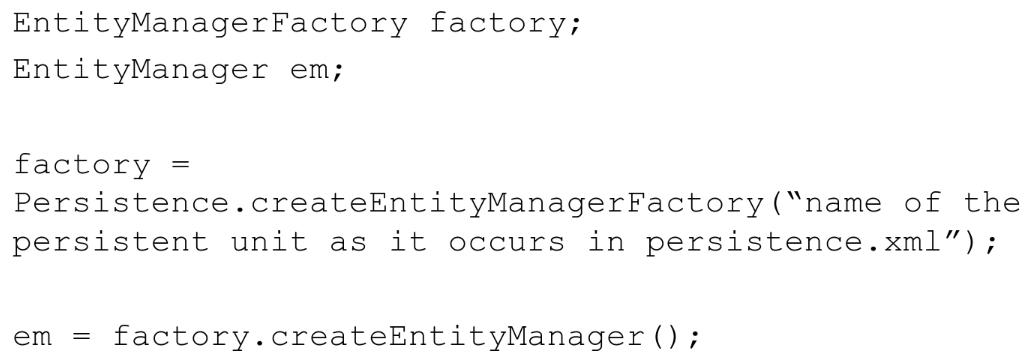
\includegraphics[width=1\linewidth]{images/entity_manager_factory.png}
    \caption{Creazione di un'Entity Manager tramite una Entity Manager Factory.}
    \label{fig:ent_man_factory}
\end{figure}

Per poter tenere traccia dei cambiamenti, però, essa deve poter essere a conoscenza sia della presenza in memoria degli oggetti che di eventuali cambiamenti apportati ad essi: bisogna quindi capire se il tipo di policy di notifica della UoW adottato è Caller Registration o Object Registration.\\
Nel caso di JPA, la creazione o distruzione di un oggetto deve essere segnalata dalla logica di business (Caller Registration), mentre i cambiamenti effettuati agli oggetti sono rilevati automaticamente (Object Registration).

I cambiamenti vengono però rilevati automaticamente solo se gli oggetti sono effettivamente monitorati dalla Entity Manager, ovvero la logica di business si è occupata di segnalare la loro presenza in memoria.
Un oggetto di una Entity Class può quindi trovarsi in due stati:
\begin{itemize}
    \item managed: la logica di business ha comunicato il caricamento in memoria dell'oggetto all'Entity Manager, e l'oggetto è quindi monitorato.
    \item unmanaged: l'Entity Manager non è a conoscenza dell'oggetto. Possono quindi essere presenti in memoria più copie dello stesso oggetto \footnote{La copia monitorata dall'Entity Manager e una o più copie non monitorate.}, portando a inconsistenza e impossibilità nel rendere persistenti i cambiamenti.\\
    Questo caso si verifica principalmente nei sistemi distribuiti, quando la macchina riceve un oggetto dalla rete.
\end{itemize}

\subsubsection{Operazioni offerte da una Entity Manager}
Le principali operazioni offerte da una Entity Manager sono:
\begin{itemize}
    \item \verb|persist|: rende persistenti le modifiche apportate agli oggetti managed. In realtà, le modifiche non vengono immediatamente rese persistenti, ma solo schedulate.
    \item \verb|flush|: rende immediatamenti persistenti le modifiche apportate agli oggetti managed.
    \item \verb|find|: dato l'ID di una risorsa nel database, restituisce una reference al relativo oggetto in memoria. Se l'oggetto non è presente, allora lo carica completamente, ovvero tutti i campi sono inizializzati correttamente. L'oggetto caricato sarà in uno stato managed, ovvero monitorato dalla Entity Manager;
    \item \verb|getReference|: identico all'operazione di \verb|find|, ma l'oggetto viene caricato in maniera lazy;
    \item \verb|merge|: dato un oggetto non ancora monitorato dalla Entity Manager, permette di rendere l'oggetto managed. Se è già presente un oggetto managed con lo stesso ID di quello specificato, allora l'oggetto monitorato assumerà i valori di quello ricevuto in input dalla \verb|merge|;
    \item \verb|remove|: dato un oggetto managed, rende l'oggetto unmanaged e schedula la sua rimozione dalla memoria.
    \item \verb|refresh|: dato un oggetto, cancella tutte le modifiche apportate a quell'oggetto e non ancora rese persistenti. Per farlo, ricarica dal DB la risorsa con l'ID specificato.
\end{itemize}

\subsection*{Mapping e annotazioni}
Gli oggetti in memoria e le risorse nel database devono mantenere un mapping consistente. Per farlo, JPA offre le annotazioni, particolari "suggerimenti" specificati dal programmatore nelle Entity Class che permettono alla Entity Manager di capire come un oggetto si traduce nel database.

Le annotazioni sono molte. Le più importanti sono:
\begin{itemize}
    \item \verb|@Entity|: posto prima della signature di una Entity Class, specifica che l'oggetto è mappato in una tabella del DB con lo stesso nome e la stessa struttura della Entity Class.
    \item \verb|@Table(name="...")|: posto prima della signatured di una Entity Class, specifica che l'oggetto è mappato in una tabella del DB di nome \verb|...| e con la stessa struttura dell'oggetto.
    \item \verb|@Id|: posto prima del campo della Entity Class che identifica l'Identity Field.
    \item \verb|@Column(name="...")|: posto prima di un campo della Entity Class, specifica che il campo è mappato in una colonna di nome \verb|...| nella tabella associata alla Entity Class.
    \item \verb|@SecondaryTable(name="...", @pkJoinColumns(@PrimaryKeyJoinColumn(name="...")))|: l'oggetto è mappato in due tabelle del DB, il cui nome della prima è quello della Entity Class, il nome della seconda è invece quello specificato nell'annotazione. L'oggetto corrisponde quindi a una join delle due tabelle.
\end{itemize}

\subsubsection{Mappare la cardinalità delle relazioni}
Le Entity Class possono essere in relazione tra loro, e ognuna di queste relazioni può avere una sua cardinalità.
I quattro tipi di relazioni sono:
\begin{itemize}
    \item uno-a-uno. In questo tipo di relazione, un'Entity Class possiede un campo contenente un singolo oggetto dell'altra Entity Class.
    Nel database, le due entità sono invece memorizzate in due tabelle diverse, e sarà necessaria nell'entità principale una foreign key alla primary key dell'entità secondaria.\\
    L'Entity Manager rileva questo tipo di relazione grazie a due annotazioni:
    \begin{itemize}
        \item \verb|@OneToOne|
        \item \verb|@PrimaryKeyJoinColumn|: specifica che il campo dell'entità principale si traduce in una foreign key alla primary key dell'entità secondaria.
    \end{itemize}
    \item molti-a-uno. FINIRE
    \item uno-a-molti. In questo tipo di relazione, un'Entity Class possiede una collezione di oggetti di un'altra Entity Class.
    Nel database, la tabella associata all'Entity Class secondaria contiene tutti i record contenuti nelle collezione. Ogni record contiene però anche una foreign key alla primary key del record nella tabella associata all'Entity Class principale che rappresenta l'entità che possiede la collezione.
    \item molti-a-molti. FINIRE
\end{itemize}